\chapter{Implementation of an Unobtrusive Prototype}
\label{chapter:implementation}

During our research on social navigation we came in contact with
\abbr{SINTEF}%
\sidenote[5]{
  \abbr{SINTEF}\dash{}headquartered in Norway\dash{}is
  the largest independent research organization in Scandinavia.
}
and their \abbr{RECORD} research project.%
\abbr{RECORD} is a research project which
  \postquote{record08}{%
    aims to provide knowledge and methodologies to improve development of
    online community products and services}
One of the partners of this project is \abbr{NRK}%
\sidenote[6]{
  The Norwegian Broadcasting Corporation.
}
with their \urort{} web site. After some coordination meetings with the
\abbr{RECORD} project it became clear that \urort{} and its web site
would be an excellent candidate for trying out social navigation techniques.

As we'll see in the next section, it's possible to build applications on top
of existing web sites by creating unobtrusive implementations.
Following the background information on building applications
on top of established web sites we give an account of
what kind of navigation system we wanted to build for \urort{}, go on to
describe why we decided on such navigational designs, and conclude with an
explanation of the deeper technical decisions we had to make.
\appendixref{selection.of.third.party.software},
describes what kind of third party software we used for realizing the
implementation details we describe in this chapter.

\section{Building on Top of the Web}
\label{section:implementation.building.on.top.of.the.web}

Going in and making changes to an existing web site can be both an
daunting and time consuming task. First one have to establish a trustworthy
relationship with the creators of such a site so they can be certain
you're not introducing bugs in their production software. Secondly, grasping
the code base, third party libraries, and development tools of such a software
project demands a lot of upfront effort before any real development work can
begin. This goes against the prototypical process we intended to use while
experimenting with \urort{}.

Even though we've had an ongoing dialog with the developers of \urort{}, we
decided to create our prototype as a layer on top of their site.
By using an
extension
for a leading open source%
\sidenote{
  The \project{Firefox} web browser. Available at \url{http://firefox.com}.
}
web browser we were able to create a script which
made changes to the way \urort{}
were presented to users who were participating in our study.
Such an approach would hopefully result in a transparent experience for our
end users, as long as they had taken the necessary steps to set up 
our script.

\subsection{Inspiration}

The idea of creating additional features for a web site in this manner
came from the author's involvement in an underground community based around
the Ruby programming language. \project{Hoodwink.d}%
\sidenote[-1]{
  Hoodwink.d's starting point for new users can be seen
  at \url{http://hoodwinkd.hobix.com}.
}
is a service that lets members post comments on all kinds of
web sites. These comments are only visible to the members of the
community.

\begin{figure}
  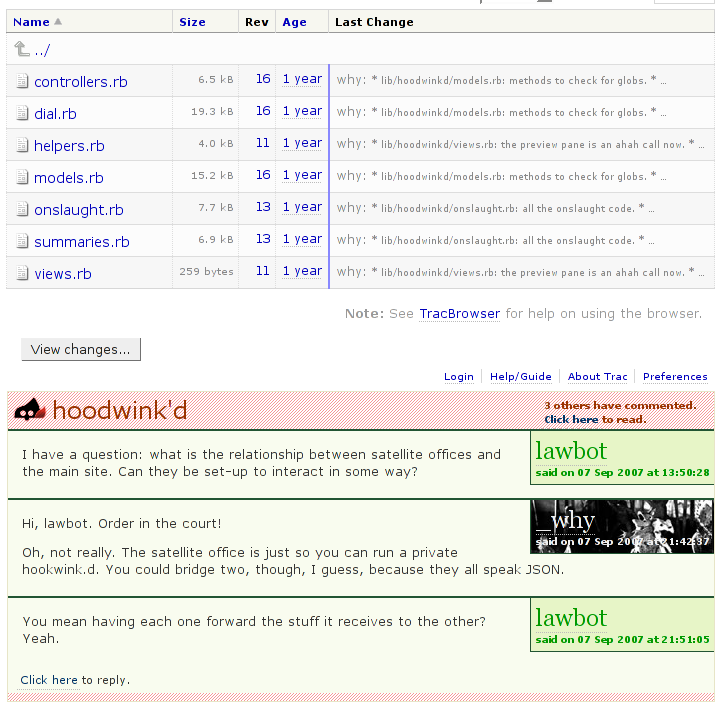
\includegraphics[width=\textwidth]{scrsh_hoodwinkd_comment_source}
  \caption[Hoodwink.d Comments]{
    Comments on the repository browser of Hoodwink.d's source code,
    retrieved March 7, 2008, from
    \url{http://code.whytheluckystiff.net/hoodwinkd}
  }
  \label{figure:scrsh.hoodwinkd.comment.source}
\end{figure}

The really interesting part of Hoodwink.d is the features
it enables on top of the Web. One can create a comment visible only to the
community's members on any web page that is supported. This support is not
dependant on the creator of the web site. The users of Hoodwink.d need to
record some information of the web site (where the comments should be placed)
to make it supported. \figureref{scrsh.hoodwinkd.comment.source} shows an
example of how these comments are displayed on a web page.
This page does not natively support
comments. Using Hoodink.d for such means is a very cheap (time wise) option
compared to implementing commenting in the web site itself.
They are perceived as being part of the web page, even though they
are inserted right after the page is fully loaded.

\section{Design}
\label{section:implementation.design}

With design, we mean how the application we're making is
presented to users. For discussion of how the software is designed
or architected internally, take a look at
\sectionref{implementation.architecture}.

\subsection{Philosophy}

Our philosophy when creating a navigational design have been
similar to that practiced by
\begin{fullquotation}[\chap{3}]{exupery67}{in aviation design}
  \noindent
  And now, having spoken of the men born of the pilot's craft, I shall say
  something about the tool with which they work, the airplane. Have you
  ever looked at a modern airplane? Have you followed from year to year
  the evolution of its lines? Have you ever thought, not only about the
  airplane, but about whatever man builds, that all of man's industrial
  efforts, all his computations and calculations, all the nights spent
  over working draughts and blueprints, invariably culminate in the
  production of a thing whose sole and guiding principle is the ultimate
  principle of simplicity?

  It is as if there were a natural law which ordained that to achieve this
  end, to refine the curve of a piece of furniture, or a ship's keel, or
  the fuselage of an airplane, until gradually it partakes of the
  elementary purity of the curve of a human breast or shoulder, there must
  be the experimentation of several generations of craftsmen. In anything
  at all, perfection is finally attained not when there is no longer
  anything to add, but when there is no longer anything to take away,
  when a body has been stripped down to its nakedness.
\end{fullquotation}

This philosophy is closely related to minimalism.%
\sidenote{
  Minimalism is a movement where the
  infamous architect Mies van der Rohe popularized the concept of
  \q{less is more}\dash{}achieving the maximum effect with the minimum of
  means \citep{whitman69}.
}
We feel the prototype we're creating should provide users
with only the necessary information for affording navigational behavior.

\citet{schwartz04} wrote a book called
\work{The Paradox of Choice: Why More Is Less} where he explains that
we in our modern society have an overabundance of choice. All these choices
can produce psychological distress. As \citeauthor{schwartz04} explains this
problem can be resolved by limiting the amount of choices we are presented
with.

Our design could potentially introduce even more choices. We're
introducing more information, and more navigational choices, into the
\urort{} web site. A possible solution could be to remove some of the
choices presented to the user if we felt the choices we're providing
for navigation were of higher importance than those provided by
default. We decided against this since we wanted to test our navigational
design in opposition to the navigational designs already provided. By
eliminating some of the default navigation we would not be sure
if potentially more satisfied users was the result of our removal of
choices, the new choices we provided, or a combination.

\subsection{Activity stream for \urort{}}
\label{section:implementation.design.activity.stream}

According to \prequote[\p{193}]{dubinko07}{}{%
  There is enormous and growing interest in the consumption of
  up-to-the-moment streams of newly published content of various forms: news
  articles, posts on blogs or bulletin boards, and multimedia data such as
  images, songs, or movie clips}

In the \urort{} web page there is currently not an easy way to discover what
is new for the areas that you personally care about. The main page
as seen in \figureref{scrsh.urort.main.page}
displays the latest editorial articles. In some sense these activities
represent new content. At the right margin there are also lists of both
editorial song selections and the most popular by listenings and downloads.
Whether you're
logged in to the web page by a registered user handle or browsing the page
anonymously, you're presented with the same information. Navigating onto your
personal profile page yields the same results: no good pointers to fresh
content which you are likely to especially care about.

\begin{figure}
  \begin{whole}
    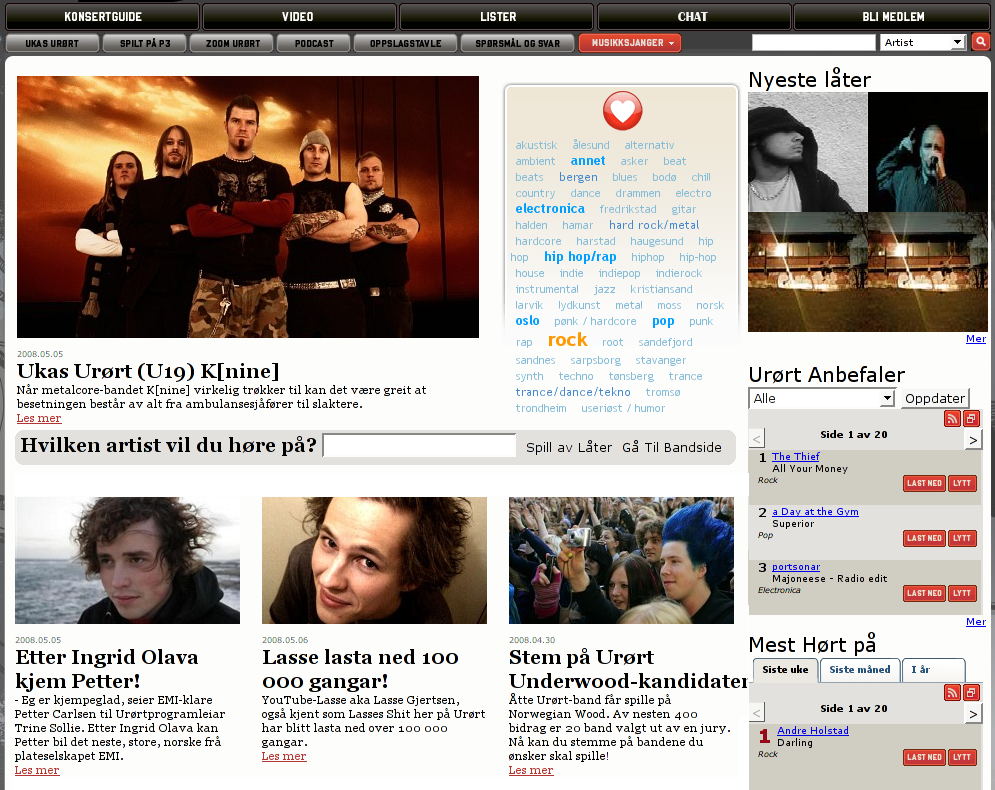
\includegraphics[width=\wholewidth]{scrsh_urort_main_page}
    \caption[\urort{} Main Page]{
      The main page of \urort{} with mostly editorial content.
      Retrieved May 8, 2008, from
      \url{http://www11.nrk.no/urort/default.aspx}.
    }
    \label{figure:scrsh.urort.main.page}
  \end{whole}
\end{figure}

When we conducted our study of the Facebook social network site we became
intrigued by how easy it was to keep updated on the latest developments for
our friends by using its news feed, as described in
\sectionref{analysis.facebook.news.feed}. 

\newcommand{\placefriendfeed}{%
  \sidefigure[FriendFeed Activity Stream]{%
    Activity stream for the author on FriendFeed,
    retrieved May 18, 2008, from
    \url{http://friendfeed.com/uggedal}
    \label{figure:scrsh.friendfeed.me}
  }{%
    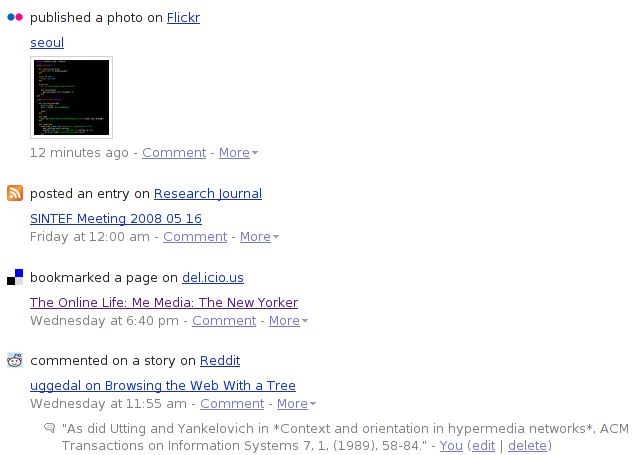
\includegraphics[width=0.9\marginparwidth]{scrsh_friendfeed_me}
  }
}

Such streams of activity seem to have become popular also outside Facebook.
\project{Socialthing!} and \project{FriendFeed} are two services that
aggregates such streams from several sources and provides an unified stream.
Their distinguishing factor is that Socialthing! fetches activities for your
\placefriendfeed%
existing friends on services as Facebook and Flickr. FriendFeed on the other
hand only collect activities from the people you decide to follow on
FriendFeed itself. FriendFeed can in addition display your personal stream
as an aggregation of all supported services you're using. Both activity stream
aggregators are shown in \figureref{scrsh.friendfeed.me} and
\figureref{scrsh.socialthing}.

\begin{figure}
  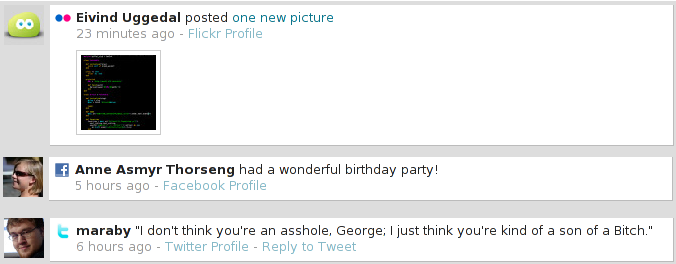
\includegraphics[width=\textwidth]{scrsh_socialthing}
  \caption[Socialthing! Activity Stream]{
    Activity stream for the author and his friends on Socialthing!,
    retrieved May 18, 2008, from
    \url{https://socialthing.com}
  }
  \label{figure:scrsh.socialthing}
\end{figure}

When the news feed was introduced on Facebook in September 2006 users
immediately responded negatively since they felt their privacy was
compromised. Even though all data available through the news feed had
previously been available to the same users, the aggregated and efficient
display of this information led to concerns \citep[\pp{13}{14}]{boyd08}. 
Interestingly these negative first reactions seemed to vanish as
\postquote[\p{19}]{boyd08}{%
  Users quickly adjusted to the new architecture; they began taking actions
  solely so that they could be broadcast across to Friends' News Feeds}
\citet[\p{1031}]{joinson08} found that the news feed was indeed used by
241 respondents to a usage survey conducted by the author. He feels these
results indicate a greater acceptance of the news feed today compared to when
it was introduced. An ethnographic study conducted by
\citet[\p{3126}]{chapman08} of several social network sites
including Facebook found the news feed to be one of the primary means of
interacting with the web site.

Based on both our own observations and other's of the perceived usefulness
of activity streams, we decided on using such a navigational design in
our prototype implementation for \urort{}.

\subsubsection{Relevant activities}

The approach seen at Facebook for letting users know what's fresh and relevant
through an activity stream (or news feed as Facebook calls it)
seemed a good fit for \urort{}. But
\urort{} does not have the concept of friends as seen in social network sites.
\urort{} exists for people to freely share their music and let others find
music they like\dash{}and not making new friends or keeping in touch with
old friends. How do we then find recent activities which potentially could be
interesting for our users when we don't have any friends to consult?

We tried to answer this question by using a feature on \urort{} that allows
any user to \emph{favor} an artist. If a user conducts such an action he or
she becomes a \emph{fan} of that artist. We don't know why people signify
artists as their favorites on \urort{}, but the main reason may be that
they simply like the music the artist is publishing.
Another reason could be that people know the artist personally and therefore
add them as a favorite\dash{}not dependent on whether they like their music or
not.

But regardless of the motives for adding an artist as a favorite it requires
a conscious effort from the user. We're therefore led to believe that the list
of artists a user have favored are more important than other artists on
\urort{}. Our design is therefore based on the activities of a person's
favorite artists. Initially we toyed with making a friend like concept on
\urort{} by saying that people which share one or more favorite artists with
you are in some way similar to yourself. We had to throw away this idea
because of technical problems with getting such a solution to scale.

\subsubsection{Activity types}

There were many activities taking place associated with an artist
which we could potentially use in our activity stream. We decided to select
those which contained information about when the activity occurred and was
technically easy%
\sidenote{
  Easy as in only requiring access to content freely available on
  \urort{}.
}
to retrieve. Those that matched our criteria was:

\begin{items}
  \iterm{Songs} being published by an artist.
  \iterm{Song reviews} being written by users.
  \iterm{Concerts} being performed by an artist.
  \iterm{Blog posts} being written by an artist.
\end{items}

As you can see three of these activities are conducted by artists themselves
while reviews are conducted by other users.

\subsubsection{Activity filtering}

\begin{figure}
  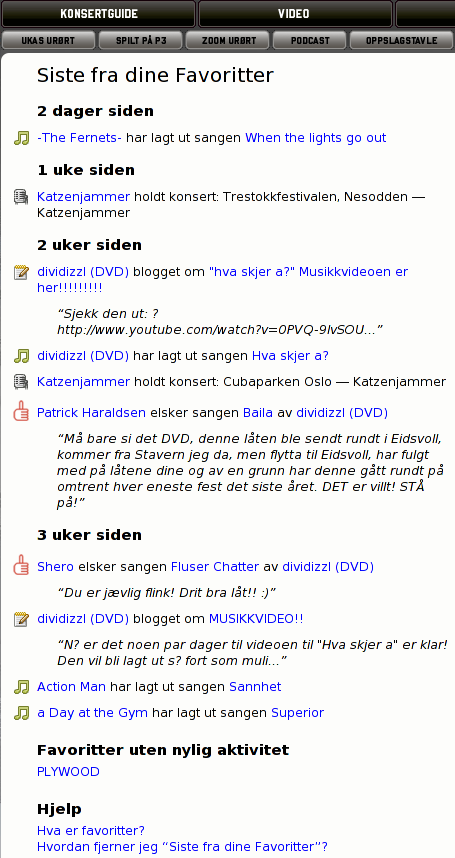
\includegraphics[width=0.65\textwidth]{scrsh_urort_activity_feed}
  \caption[\urort{} Activity Stream]{
    Activity stream for experiment users on \urort{},
    retrieved Jun 2, 2008, from
    \url{http://www11.nrk.no/urort/default.aspx}
  }
  \label{figure:scrsh.urort.activity.feed}
\end{figure}

There was quite bit of activity information available based on our four
categories for a typical artist. When a user had several artists as
favorites the amount of activity information got large. We therefore had
to filter out some activities and only show what we thought would be most
relevant.

Firstly we were only concerned with historical information in our activity
list. Future concert events were therefore filtered out. Secondly we were only
showing
the most recent activities believing that fresh content is more important than
aged content. As activities were sorted chronologically in our stream, we
simply cut off all activities after a preset number of the most recent
activities were displayed. The version of our prototype which was tested by
real world users showed only the ten most recent activities.

In the case of Facebook,
they are not showing the complete picture of friend activity in their news
feed. It's believed that up to 80\% of all recent activities are filtered
out \citep{elliott08}.
Facebook's approach for only showing a selection of recent activity is
probably driven by technical scalability problems, and not a desire to only
present a selection of the recent activity of friends. In our activity stream
we gave users a complete picture of all types of activities within the
cut-off point.

We named the implementation
\latest{}\dash{}emphasizing the focus on providing the latest activities
for a user's favorites.
The complete design of our activity stream for \urort{} can be seen in
\figureref{scrsh.urort.activity.feed}.

\subsection{Favorite list}
\label{section:implementation.design.favorite.list}

As we'll describe in
\sectionref{empirical.methodology.experiment.design}
we decided to used a control group in our experiment setting. The navigational
design we presented them with did not include an activity stream. In stead
they
were simply presented with a list of their favorites so that they manually had
to keep up with what recent activity their favorite artists were conducting.
This implementation was also named \latest{} so that it would appear similar
to the full featured version.
The design of the control group implementation can be seen in
\figureref{scrsh.urort.favorite.list}.

To give both our control and experiment group the same navigational
possibilities\dash{}excluding the activity stream\dash{}we decided to show a
list of the favorites without recent activity for our experiment group. If all
their favorites had activities present in the stream, no such list was
displayed. \figurepageref{scrsh.urort.activity.feed} shows the listing of one
such artist without recent activity.

\begin{figure}
  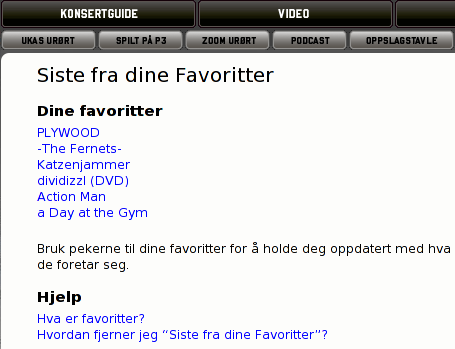
\includegraphics[width=0.65\textwidth]{scrsh_urort_favorite_list}
  \caption[\urort{} Favorite List]{
    Favorite list for control users on \urort{},
    retrieved Jun 2, 2008, from
    \url{http://www11.nrk.no/urort/default.aspx}
  }
  \label{figure:scrsh.urort.favorite.list}
\end{figure}

\section{Process}

This sections details the development process we used for building our
activity stream implementation for \urort{}.

\subsection{Prototyping}

A \term{prototype} is an early version of an application that are used for
finding out more about the problem at hand and its possible solutions
\citep[\p{409}]{sommerville06}.
The software developed for our research on social navigation fitted these
characteristics. It was not supposed to be used after its behavior was
evaluated. For that it was to inefficient and relied on specific web browser
environments and extensions. This did not mean that the prototype couldn't
have impact on how \urort{} evolved in the future. If our evaluation favored
our design decisions the developers of \urort{} could take advantage of such
potential improvements in their web site design.

\citet[\pp{409}{410}]{sommerville06} explains that a prototype can be used for
\begin{inparaenum}[(i)]
  \item gathering more sound requirements from users during a
    requirements phase,
  \item evaluating the feasibility of a proposed design during a
    design phase, and
  \item testing the final system by verifying it against the prototype.
\end{inparaenum}
We followed his second example of prototype usage by making a prototype
for what we believed to be a sound social navigation design. This was then
evaluated. If time had permitted (sadly one has limited time and resources
available during master thesis research) the results of such an evaluation
could have been input in a new design process and a new prototype system.

As \citet[\p{114}]{mcconnell04} explains, prototyping can mean different
things based on context. Often it's used to explain systems where one writes
the least amount of code to get a solution and throw it all away when the
design question is answered. This was not our intent. We tried to make the
system fully operational and make the code we authored comprehensible and
valid. More precisely we were creating a \term{high-fidelity} prototype
\cite[\p{78}]{rudd96} with a robust architecture.

The reason for creating a robust application was twofold. Firstly we were
developing
the prototype as part of our master thesis and it was meant to show how
proficient we were in both programming and designing applications. We
imagined delivering a barely working and poorly constructed software package
would not be beneficial for our examination results.
Secondly the application could potentially see some stress under user testing
depending how large the test population were. Having a crashing or
non-functioning application during such testing could have proved to be costly
with regards to our experiment results.

We did therefore create a prototype to demonstrate our ability (or inability)
to develop software. This was not our sole reason, and probably not the most
important. As \citet[\p{292}]{mayhew90} describes, prototyping is not
successful if one have not learned something during the process about what one
set out to investigate at the outset. We wanted to investigate navigational
designs and the prototype was with such a focus nearly a means to an end.

\subsection{Testing}
\label{section:implementation.process.testing}

One can verify that the application one are building functions as it's
supposed to do as code is added and changed by using automated tests.
We have personally experienced benefits with using automated testing on
earlier projects.
\term{Test-driven development} is a development technique
where one writes an automated test for a non-existent feature or
improvement before one actually implement the feature itself\dash{}development
is literally driven by tests. So the focus is not primarily on the test, but
to better design software through a test-first approach.
\citet{janzen08} conducted studies
on both developers in companies and university students for finding out
whether a test-driven approach improved the quality of software design.
Groups which wrote a test before the accompanying code were measured
against groups which wrote their test after implementing the solution.
They found that code size decreased when a test-first approach was
used\dash{}both classes and methods were smaller and simpler. In addition
test-first developers had better coverage of the implementation code in
their tests \citep[\p{81}]{janzen08}. This could indicate that it's
easier to opt out from testing after you have a piece
of working code. The discipline that test-driven development dictates
makes it impossible not to write tests.

\term{Behavior-driven development} is a response to the test-driven
development approach. It was introduced by \citeauthor{north06} for shifting
the focus from writing tests to writing specifications of behavior
\citep{north06}. By writing specifications one is able to
more clearly describe the intent of an application than when one
are writing traditional tests.

We were convinced of the benefits of behavior-driven development based on
earlier development projects and were therefore developing our
prototype application with such a development process. Having specifications
that could be automatically run to check how our application conformed to our
expectations was very valuable. This was especially so when working
with \urort{} as an external data source since we did not have control over
the stability of its structure.

\section{Architecture}
\label{section:implementation.architecture}

Our implementation basically needs to do two things:

\begin{enum}
  \item Collect existing data from various places on the \urort{} web site.
  \item Display this data in existing web pages on the \urort{} web site in
    a way that we hope will enhance navigation.
\end{enum}

\subsection{Extending an established web site}

As we've described earlier in this chapter we're creating a prototype
application. Inspired by solutions in the Hoodwink.d community we set
out to implement our system on top of already established web pages.

\citet{laird07} makes a case for using the means of such a browser
extension\dash{}Greasemonkey\dash{}and custom scripts for
realizing projects that without such technology would
never have come to existence. As he describe there is a sweet spot where such
an approach really shines. He therefore created a framework for determining
if a given project embodies the factors that would make this kind of an
implementation a particularly suitable solution. What follows is a recitation
of his selection factors and how our project adheres to these.

\subsubsection{Do you have access to the source code of the web application?}

When the source code of the target web site is available it would probably
be easier to just change that. The case is made for using Greasemonkey when
the source code is not available. Since we don't have access to the internals
of \urort{} we see this factor as favorable for Greasemonkey in our project.

\subsubsection{If the application is under your control and source code is
  available, is updating the application a risky endeavor?}

This factor does not apply to our implementation since we obviously did not
create \urort{} ourselves. Had we done that we could have used
Greasemonkey for adding new features without putting the existing web
site in danger as it would be externalized from the original implementation.

\subsubsection{How critical is the feature to be added?}

If the web site is not functional or complete without the new feature
it is advisable to defer from using Greasemonkey. The reason is the
difficulty of ensuring that all users have the extension installed
and the newest version of the custom script. Since we will be able
to ensure that our test users have the right extension and scripts
installed this is of no concern to us. In addition \urort{} is
functioning fine without our feature enhancement which makes
Greasemonkey a sound technical solution for our means regarding this factor.


\subsubsection{Is Firefox available for the potential users, and does it
  work with the target application?}

The Firefox web browser should be available to install on most platforms
and we can report that it works fine on the target web site.
We cant expect all potential users to install Firefox on their
computers. This limits the reach we have with a Greasemonkey based
implementation.

\subsubsection{To what degree are the target users computer literate?}

Installing a web browser, an extension for it, and finally a custom script
can be a bit complicated for certain users. We have to expect the
test users to be a selection of our general population and some could
therefore have trouble with achieving such a setup. On this aspect
a solution that alters the original application would work better
since users are not required to change their computing environment.
We hope to partly solve this problem with providing clear instructions
for how users can configure their environments to support custom
Greasemonkey scripts.

\subsubsection{What size is the user population that needs the new feature?}

This factor is based around the fact that server applications can be more
easily updated since they seldom require intervention by the user. It's
much harder to ensure that client applications like Greasemonkey are
kept up-to-date by its users. It's argued that such an approach works
better for smaller populations and one should therefore keep users
of custom Greasemonkey scripts to a minimum.

Since we're not foreseeing the use of our implementation outside user
testing the application does not have to be kept up to date. In addition
we're anticipating a fairly limited user base due to our test setting.
Greasemonkey should therefore not put any hindrance in place for
our implementation in relation to this factor.

\subsubsection{Is the application exposed to the public internet?}

This factor relates to the previous about keeping the user base limited.
In addition to limiting the size of your user population it's also
important to know them\dash{}know who your users are\dash{}so that
one more easily can support them if need be. Since our application
only will be available to test users we see no disadvantage to
using Greasemonkey in this regard.

\subsubsection{How often is the page structure in the web application
  changing?}

Since implementations based around Greasemonkey often is dependent on the
underlying web site and its structure it's important that this remains
stable while the implementation is in use. While we in our project
will have a fairly small time window of actual use we've been concerned
that changes could break our implementation.

We see two possible solutions for this problematic aspect of Greasemonkey
implementations. Firstly communication between the developers of
\urort{} and ourself about upcoming changes would allow us to anticipate
them and handle them gracefully when they arrive. Secondly one could
introduce a meta structure in the web site by using agreed-upon
class names of certain \abbr{HTML} elements in the style of
what \term{microformats}%
\sidenote{
  Microformats are a set of simple and open data formats for better
  structuring of web content. All microformats adheres to the
  principles of solving a specific problem, starting as simply as
  possible, being designed for humans first\dash{}machines second,
  reusing elements from already established standards
  being modular and embeddable, and encouraging decentralized development,
  content, and services \citep[\p{7}]{allsopp07}.
  To us the essence of microformats seems to be the usage of semantic class
  names in \abbr{HTML} elements. By semantic class names we mean naming
  classes for what the elements they belong to represent.
}
are trying to achieve.

\subsubsection{Does the application manage or expose sensitive information?}

Because of the architecture of Greasemonkey, scripts written for the extension
can be vulnerable to attacks if the developer is not careful. It's
therefore not advisable to use Greasemonkey for highly sensitive web sites.
This is not a concern for our project as all the information handled by our
application can be found publicly on the \urort{}
web site.

\subsubsection{Does the new feature require many changes to the existing web
  application?}

Using Greasemonkey to enhance and alter existing web pages is not as straight
forward as altering the source of the web page. Therefore massive changes to
an existing web site is best handled directly in the source code leaving
Greasemonkey to be the better alternative when only smaller alterations and
addition are needed.

The changes we propose to introduce in the \urort{} web site is not earth
shattering in scope and size. We therefore believe and hope our implementation
can be implemented without too much additional effort with Greasemonkey.

\subsubsection{Does the target web application already have JavaScript code
  that mutates the page?}

This factor tries to capture the fact that the behavior implemented with
custom Greasemonkey scripts are run before any additional behavior
implemented in the web site itself. It's therefore hard to manipulate
a web site that mutates over time.

In our project we seem to be quite fortunate as we're only planning on adding
behavior to the \urort{} web site, not changing any existing behavior.
We therefore don't have to concern ourselves with some of the dynamically
already present on \urort{}.

\subsubsection{Does the feature require communication with a server in a
  different network domain than the web application?}
\label{section:implementation.architecture,extending.different.domain}

Standard web pages can asynchronously retrieve information through using
JavaScript and the \code{XMLHttpRequest} object. To enforce a certain
level of security browsers does not allow such requests to retrieve
information from other domains than what the request was sent from.
This limitation is eliminated in Greasemonkey scripts as one can request
information from other domains through a similar asynchronous request object
existing in the extension.

This feature is vital for our project. As we'll see in the next section we're
dependent on requesting information from a resource that we ourself have
control over from the custom Greasemonkey script. This resource is however
not hosted in the domain that \urort{} is operating within. Without
cross-domain requests in Greasemonkey our implementation would be infeasible.

\parabreak

Based on how our project positioned itself with regard to the important
factors for the feasibility of using Greasemonkey
according to \citet{laird07}, we have to say that we
don't see any major objections for doing so.
We believe the benefits of a prototype implementation
based on Greasemonkey outweighs the disadvantages with such a technical
solution.

Another solution would be to create a web proxy that altered pages specific to
\urort{}. \citet[\p{1109}]{keller97} took this approach when developing
a collaborative bookmarking service. As the authors explain a proxy-based
solution ensures universal access across browsers and platforms requiring no
installation of additional browser extensions or plugins. The drawbacks to
such and approach for our prototype is quite clear. A user having enabled
our hypothetical web proxy would have to take a round trip to our server for
every web page he or she visited, regardless of whether it was \urort{}
related. This would introduce substantial loads on our servers and users would
probably notice reduced page load times when browsing the Web.

\subsection{Client-server model}

A client-server model is an architecture where one is separating a system into
two logical parts:
one or more clients and one or more servers \citep[\p{3}]{lewandowski98}.
The client is a \openpostquote[\p{11}]{malkin96}{%
  computer system or process that requests a service of another
  computer system or process}
and the server is a \postquote[\p{49}]{malkin96}{%
  provider of resources}
More specifically a client presents the user interface, uses a predefined
language for querying the server, communicates these queries through a given
communication method, performs computation on the the results of queries send
by the server, and displays these through the user interface
\citep[\pp{78}{79}]{sinha92}. A server is characterized by providing a service
to the client, responding to queries constructed by the client,
and hiding away its underlying technical system for the client
\citep[\p{79}]{sinha92}.

The client and server thus have disparate responsibilities\dash{}the client is
a consumer and the server is a producer \citep[\p{3}]{lewandowski98}.
This delegation is the
essential part of client-server computing and enables one to focus on one
aspect of a problem as one does when adhering to the concept of
\term{separation of concerns} \citep[\p{61}]{dijkstra82}.
A client-server model also enables one to scale both horizontally and
vertically%
\sidenote[-1]{
  To scale horizontally entails adding more servers to a client-server
  architecture. When one increases the resources of a single server
  one is scaling vertically.
}\dash{}an
impossible feat with monolithic systems \citep[\pp{7}{8}]{lewandowski98}.

We therefore decided to use a client-server architecture so that we could
offload some of the more computationally expensive operations off the client
and onto a dedicated server. Another benefit of such an architecture is that
it allows us to cache data globally\dash{}shared by all clients. This means
that data collection is handled on the server-side, while data display
obviously is handled on the client-side.

Following the characterization of client-server systems provided by
\citeauthor{sinha92} our client is presenting a user interface
by altering the structure of the \urort{} web page. The client sends queries
to the server in the form of \abbr{HTTP}%
\sidenote[-1]{
  Short for Hyper Text Transfer Protocol\dash{}the
  protocol used for transferring data on the Web.
}
formatted requests. Our server takes these queries in \abbr{HTTP} form
and goes to the \urort{} web site to collect the data it needs. Based on the
data the server finds at the external \urort{} web site the server does some
computations on the data before a response is sent
with the \abbr{HTTP} communication method to the client. The client take this
data (which is represented in a predefined format) and uses it to alter the
user interface by introducing new information.

\citet[\p{887}--888]{nishimoto06} implemented a system for re-finding places
one have already visited on the Web. What's interesting about their system is
that their architecture is strikingly similar to our own. They use a
client-server model with a Greasemonkey enabled browser as their client. The
client facilitates the users as they're navigating by supplying additional
information alongside existing web pages. One of the ingredients in helping
users in their browsing is suppling information from third party content
providers. By separating this computationally heavy part of the application
into the server-side they were able to offload the clients in a similar
manner we intended to use when fetching data from \urort{}.

\subsection{Caching}
\label{section:implementation.architecture.caching}

In the planning stages of our implementation and its early development we
decided to store all information retrieved from the \urort{} web site
in a relational database. We did some study into selecting the best
\abbr{ORM}%
\sidenote[-2]{
  \abbr{ORM}, an acronym for object-relational mapping, is
  \postquote[\p{889}]{linskey07}{%
    the technique of converting records in a relational database into
    object instances in an object-oriented programming environment}
  This is possible since \postquote[\p{2}]{marshall07}{%
    relational databases can be represented reasonably in object-based code if
    you simply think of database tables as classes, table rows as objects, and
    table fields as object attributes}
}
for connecting our application to the underlying database. We had this nice
model where the underlying relational database engine was abstracted away
and interaction to this database was done with a clear and explicative
\abbr{DSL},%
\sidenote[7]{
  \abbr{DSL} or domain-specific languages are programming languages shaped
  for a specific domain. By doing so one can offer more expressiveness in a
  limited application domain. This results in better usability
  and increased productivity within the limited domain compared to
  using a general-purpose programming language \citep[\p{317}]{mernik05}.
}
eliminating the need for constructing complex \abbr{SQL}.%
\sidenote[17]{
  \abbr{SQL} (initially named \abbr{SEQUEL}) stands for structured
  query language and is now the \latin{de facto} language for interacting
  with relational databases. It was invented by 
  \citet[\p{250}]{chamberlin74}.
}

Then we had a sudden realization when coding on the part of our application
that retrieved information from the external \urort{} web site, pushed it into
our relational database, and made our data available in a structured manner
through our \abbr{ORM} layer. It was not critical if we lost some or the
entirety of this data. We could just retrieve it again from our external
source. And since the data had to be kept up to date by retrieving the data
from our source within certain intervals, we saw no need to make it available
in a relational database. We were not trying to persist data, but rather
keeping a \term{cache}%
\sidenote[14]{
  According to \prequote{wikipedia08cache}{a cache is}{%
    a temporary storage area where frequently accessed data can be stored for
    rapid access}
}
of what we had retrieved.

As described we came to the realization that no persistent data
about activities was needed in our implementation.
We therefore sat out to find the best cache solution for our needs as detailed
in \sectionref{selection.stack.server.cache}.

We only cache one type of data in our implementation:
a chronologically pre-ordered list of all activities for a given artist.
Let us explain how this works
when user $X$ requests his list of recent favorite activities. Our system
first determines that user $X$ have artist $A$ and artist $B$ as
favorites. It then consults the cache and asks if it can get a list of
activities for artist $A$. The cache have a list of activities for artist $A$
and promptly returns it to its caller. Our system then tries to do the same
for artist $B$, but this time there is no list of activities for that artist
in the cache. This is a \term{cache miss}, and we are therefore forced to
retrieve information about artist $B$'s activities from the \urort{} web site.
From this information we calculate a new list which are stored in the cache
with a certain
\term{time to live}. The next time a request for artist $B$'s list of
activities are handled the cache should now be able to return that list
if the request were made within the time to live interval.

In our system we set a time to live of 12 hours. This means that activity
lists stored in the cache are retrievable within 12 hours.

\subsection{Persistence}

As detailed in
\sectionref{implementation.design.favorite.list}
we designed two versions of our prototype: one delivering an activity
stream and another only listing favorites. This introduced the need to deliver
two versions of the client software, one for our main experiment group and one
for our control group. To handle this we had to introduce persistence in our
application to know what kind of client software the last user received to
determine what software the next user should be provided with. This way every
second user receives a full-blown client version and the other users receives
a control version.

\subsection{Background processes}
\label{section:implementation.architecture.background.process}

With our cache architecture in place it became apparent that it was too
expensive time wise for users to retrieve the activities of all their
favorites when multiple cache misses occurred. We therefore decided to
\q{warm up} the cache by running several background processes that populated
our cache with fresh data from the \urort{} web site several times a day.

Since we had implemented persistence for the various test users of our system
and their version of client software, we simply used their unique user names
on the \urort{} web site as input to our cache warm up processes.

After testing the system casually we found a need for shortening the response
times in the event we received a request from a user with our full-blown
client software where no relevant activity lists
was present in cache. Initially we retrieved information from the \urort{} web
site for all artists that the requester had favored. Under this scheme a
user with several favorites could expect response times to be several minutes
in length. We therefore decided to deliver only the activities of the user's
first favorite if non of the activity lists of his or her favorites were
present in cache. On doing so we registered the non returned artists and put
them in to a similar background process as we used for our cache warm up. 

This means that the first time a user makes a request to our application he
or she will be presented with the activities of only his first favorite if no
other users previously requesting the system have similar favorites. After the
background processing of this user's favorites is complete he will get a full
picture of the activities of all his artist. We think this is an acceptable
price to pay for reduced latency.

\subsection{Asynchronous requests}

In the traditional style of \abbr{AJAX} applications we request information on
the client-side of our prototype asynchronous.%
\sidenote{
  While it's possible to create synchronous requests with the
  \code{XMLHttpRequest} object
  it's discouraged. With such requests the entire web browser
  will be locked while it's waiting for a response for its request
  \citep{crockford06a}.
}
This means that requests handled by the \code{XMLHttpRequest} object
are independent of other requests the browser is making\dash{}they
are non-blocking. This enables developers to create web pages where additional
data is requested after the page is loaded by a normal \abbr{HTTP} request.
This is often coupled with the ability to detect user behavior, and contents
are requested only when needed. \citet[pp.281--282]{stamey06} argues that
the increased complexity (and thereby size) of todays web pages have created
problems in perceived responsiveness for users due to network latency. They
think asynchronous request of small content items solves this
problem\dash{}bringing greater interactivity to the user. Another solution
that can be used is to move some processing into the client with
JavaScript \citep[\p{9}]{jazayeri07}

\subsection{Code structuring}
\label{section:implementation.architecture.code.structuring}

\begin{figure}
  \begin{whole}
    \includegraphics{fig_prototype_class_diagram}
    \caption[Prototype Class Diagram]{
      Diagram of classes and modules in the prototype server software.
    }
    \label{figure:fig.prototype.class.diagram}
  \end{whole}
\end{figure}

Both the client-side and server-side programming languages we used
are as we'll see in
\sectionref{selection.stack.client.language} and
\sectionref{selection.stack.server.language} \term{object-oriented}.%
\sidenote[-9]{
  The term object-orientation was coined by \citet{kay03} sometime in 1967.
  The motivations leading to object-oriented programming were mainly
  to find \q{%
    a better module scheme for complex systems involving hiding of details}
  and finding \postquote[p{514}]{kay96}{%
    a more flexible version of assignment, and then try to
    eliminate it altogether}
  The essence of object-orientation lies in the fundamental concepts of
  abstraction, classes, encapsulation, inheritance, object, message passing,
  methods, and polymorphism \citep[\pp{124}{126}]{armstrong06}.
}

Since our client software was pretty dense in code size (see
\sectionref{implementation.source.code} for details) and only had to handle
a small set of operations we did not use object oriented
features as classes and objects to structure our client code. Instead we used
functions as a partitioning scheme when implementing on the client side.
Our client side software was contained in two files\dash{}one file for each
of our two versions (control and full-featured).

\newcommand{\placefilehierarchy}{%
  \sidefigure[Prototype Server File Hierarchy]{%
    Hierarchy of the server prototype software.
    The code for producing this hierarchy listing can be found in
    \sectionref{source.code.hierarchy}.
    \label{figure:prototype.server.file.hierarchy}
  }{%
    \RaggedRight{\texttt{%
      \\
      |--rort\\
      |--|--external\\
      |--|--|--blog.rb\\
      |--|--|--concert.rb\\
      |--|--|--fetchable.rb\\
      |--|--|--artist.rb\\
      |--|--queue.rb\\
      |--|--cache.rb\\
      |--|--background.rb\\
      |--|--core\_ext.rb\\
      |--|--persistence.rb\\
      |--|--external.rb\\
      |--|--parsers.rb\\
      |--|--models.rb\\
      |--|--http\\
      |--|--|--download.rb\\
      |--|--|--api.rb\\
      |--|--models\\
      |--|--|--user.rb\\
      |--|--|--person.rb\\
      |--|--|--respondent.rb\\
      |--|--|--artist.rb\\
      |--|--rack.rb\\
      |--|--http.rb\\
      |--rort.rb
    }}
  }
}

However, on the server side we had to write more code and our code had to
handle quite a large set of operations. We therefore implemented our server
side software with the use of modules, classes, objects, and methods.
\placefilehierarchy%
A figure of how the various classes and modules are related to each other
can be found in \figureref{fig.prototype.class.diagram}.
The abstractions those constructs gave us, made it easier to
precisely handle the complexity and disparity of our solution. 
As
\begin{fullquote}[\p{864}]{dijkstra72}{puts it}
  the purpose of abstracting is not to be vague, but to create a new
  semantic level in which one can be absolutely precise.
\end{fullquote}

To make the handling of our source code easier we used a hierarchy of
directories and files that resembled our module and class constructs. One
file and possible directories was used for each module and class
as can be seen in \figureref{prototype.server.file.hierarchy}.

\subsection{Data structure}

We'll shortly summarize the data structure used in our database. We
stored informations about respondents to our survey
in a \code{respondents} table. We used a \code{id} column as
an identifier for each stored respondent; an \code{email} column for
identifying respondents in relation to their survey answers; a \code{group}
column to distinguish between experiment and control respondents; a
\code{slug} column to store the unique identifier a respondent have at
the \urort{} web site so that we can warm up our cache (see
\sectionref{implementation.architecture.background.process} for details);
a \code{requests} column to count the times the respondent requests data from
our server; and a \code{created\_at} column to keep track of when a respondent
first registered his email when downloading our client software.
\tableref{prototype.data,structure}
gives further details about the data we stored.

\begin{table}
  \begin{tabular}{lll}

    &
    Type &
    Constraints \\

    \cmidrule(lr){2-2}
    \cmidrule(lr){3-3}

    \code{id} &
    Integer &
    Auto incremented primary key \\

    \code{email} &
    Text &
    Unique, not empty \\

    \code{group} &
    Text &
    Not empty \\

    \code{slug} &
    Text &
    \\

    \code{requests} &
    Integer &
    Initial default of zero \\

    \code{created\_at} &
    Time stamp &
    \\


  \end{tabular}
  \caption[Prototype Data Structure]{%
    Prototype persistent data structure, by field name}
  \label{table:prototype.data,structure}
\end{table}

\section{Performance}
\label{section:implementation.performance}

Initially we did not architect our application with performance in mind. We
wanted to create a working prototype first and then try to increase it's
performance if need be.

\sidetable[Retrieval Time and Speed]{%
  Retrieval time and speed of a typical artist profile page (423kB in size),
  by system.
  Note that the speedup is not relative to
  the transfer speed as there is overhead in establishing a connection
  to the servers at \urort{}.
  \label{table:retrieval.time.and.speed}}{%

  \begin{tabular}{lrr}

    &
    \multicolumn{1}{c}{Speed} &
    \multicolumn{1}{c}{Time} \\

    &
    \multicolumn{1}{c}{(\abbr{MB}/s)} &
    \multicolumn{1}{c}{(s)} \\

    \cmidrule(lr){2-2}
    \cmidrule(lr){3-3}

    Development &
    0.4 &
    4.0 \\

    Production &
    10.2 &
    2.8 \\

  \end{tabular}
}

It became apparent that creating an activity stream for a user with several
favorites was very time consuming. We identified the major bottleneck to be
the actual retrieval of information from the \urort{} web page. We could not
do much code and algorithm wise to remedy this problem. The only solution
was to increase the bandwidth allowed on our internet connection.
As can be seen in
\tableref{retrieval.time.and.speed}
our retrieval times decreased as we moved to a production server with
better internet connectivity.

The next bottleneck we became aware of was also related to the cost of
retrieving web pages from \urort{}. We did some careful counting of the number
of retrieval attempts to \urort{} and were able to minimize these to a
considerably lower number.

The last bottleneck we encountered was the actual parsing of the retrieved web
pages from \urort{}. We were able to implement some minor optimizations, but
did not see any major improvements.

But the major performance gains were seen when we introduced a fast cache
solution and a system for periodically warming this cache up,
as described in
\sectionref{implementation.architecture.caching} and
\sectionref{implementation.architecture.background.process}.
With these two pieces in place we felt we could present users with bearable
response times.

\section{Source Code}
\label{section:implementation.source.code}

We'll wrap up the discussion of our implementation with showing some
statistics related to our source code:

\begin{table}[h]
  \begin{tabular}{lrrrr}

    &
    &
    \multicolumn{3}{c}{Number of lines of} \\

    &
    \multicolumn{1}{c}{Files} &
    \multicolumn{1}{c}{code} &
    \multicolumn{1}{c}{comments} &
    \multicolumn{1}{c}{blank lines} \\

    \cmidrule(lr){2-2}
    \cmidrule(lr){3-5}

    Client implementation &
    2 &
    373 &
    42 &
    87 \\

    Server implementation &
    21 &
    850 &
    9 &
    189 \\

    Server specification &
    16 &
    714 &
    0 &
    179 \\

  \end{tabular}
  \caption[Prototype Source Code Statistics]{%
    Prototype source code statistics, by type}
  \label{table:prototype.source.code.stats}
\end{table}

By dividing our number of lines of specification code with implementation code
we get a ratio of 84:100
\begin{sparkline}{3}
  %Name  Size Unit
  %Spec   84%  .84
  %Code  100%  1
  \sparkspike .25  .84
  \sparkspike .75  1
\end{sparkline}
between specification/implementation on the server side.
